
\section{\deltaE}
\label{sec:delta}

To enhance the storage efficiency of compressed models, we introduce a \deltaE that stores the differences between successive checkpoints. Delta encoding works well with quantized models, tracking changes between quantization buckets rather than exact values.


\noindent\textbf{Calculating Delta.} To compute the delta between the adjacent checkpoints, we transform quantized values into integers and calculate the difference between the quantized integer values of the successive checkpoints for each layer.
We employ the technique proposed in QD-compressor~\cite{QD} that treats the quantization range as a cyclic buffer. Concretely, for integer-mapped quantized checkpoints $C^{i-1}_q$ and $C^i_q$, we compute the delta $D_i$ as $ D_i = (C^{i-1}_q - C^i_q) \text{ mod } B$, where $B$ is the number of quantization bins. %


Due to the dynamic changes in the system configuration, the number of quantization bins may vary between checkpoints. We address this by adjusting the size of the cyclic buffer to the maximum number of bins in either checkpoint. Additionally, pruned and protected values in our quantization scheme are treated as unique quantization levels with the same delta calculation. The protected values from checkpoint $C^i$ are stored separately to aid reconstruction.


\noindent\textbf{Encoding Delta.}
After delta calculation, we use a combination of run-length encoding \cite{rle} and Huffman \cite{huffman} encoding to reduce its storage footprint. Given that parameter changes are minimal in the later training stages, run-length encoding is particularly effective for compression. Standard run-length encoding can incur significant overhead due to the values with a run-length of one. We can reduce this overhead by only storing the run-lengths only when it is greater than one. However, this requires a mechanism to distinguish between the encoded values and their run-lengths. We achieve this by simply negating the sign of all the values, such that all the run-lengths are positive while all delta values are less than or equal to zero. Huffman encoding is then applied to the run-length encoded data for further compression.


\begin{figure}
    \centering
    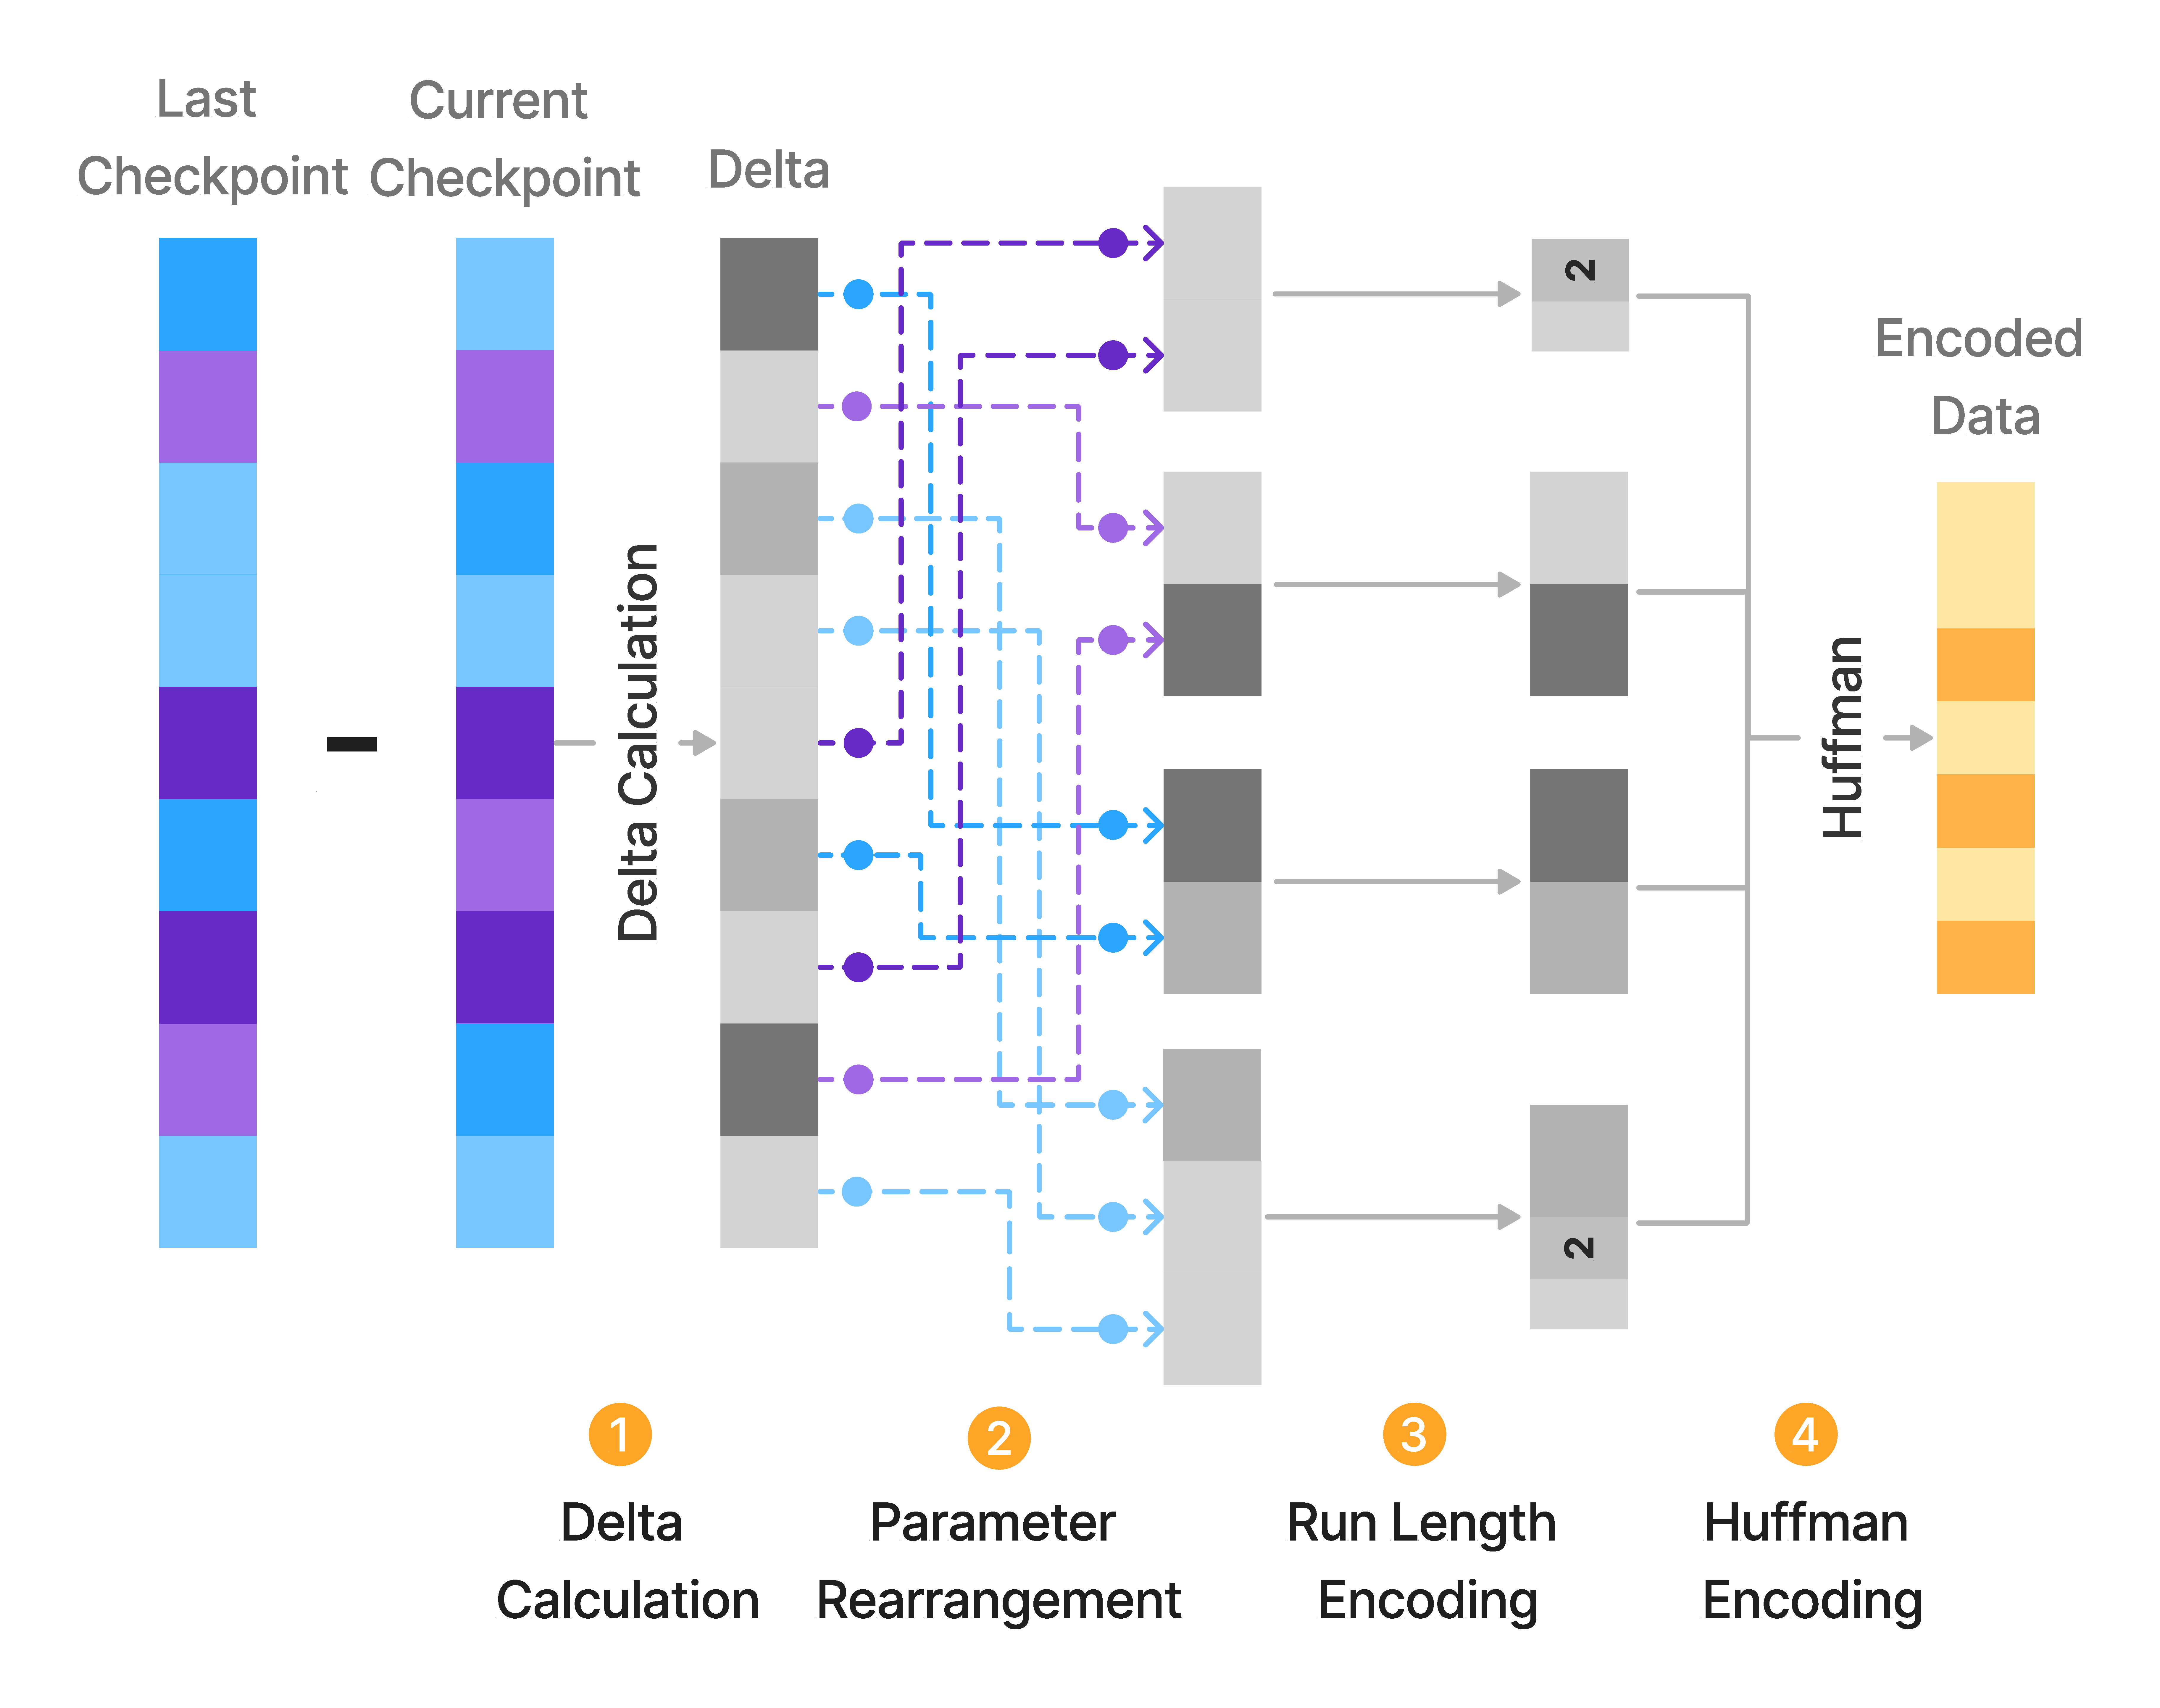
\includegraphics[width=0.95\linewidth]{figures/solution/delta_computation_v5_img.pdf}
    \caption{\small{{Rearrange and split computed delta based on the quantization bucket each parameter belonged to in the last checkpoint.%
    }}}
    \vspace{-1.5em}
    \label{fig:delta}
\end{figure}


\noindent\textbf{Optimization: Parameter Rearrangement.}
\label{sec:param-rearrangement}
The efficiency of run-length encoding depends on the arrangement of the parameters. We observe that the \emph{migration rate} (i.e., the fraction of parameters that change the quantization bucket between adjacent checkpoints) of parameters can differ significantly between different quantization buckets. In the default arrangement where parameters of all quantization buckets are interleaved, the run lengths get interrupted by the buckets with high migration rates, resulting in poor compression.

To prevent this, we rearrange parameters to isolate the parameters from different quantization buckets. After calculating the delta, we split delta values corresponding to each quantization bucket in the source checkpoint into separate groups, as shown in the second step of \cref{fig:delta}. Each group is then encoded separately. This ensures that quantization bins with high migration rates don't affect others. The process can easily be reversed during reconstruction and does not require any additional storage to obtain the parameter arrangement. \cref{algo:param-rearrangement,algo:param-reconstruction} provide a sketch of this algorithm. The approach is particularly useful when the number of quantization bins changes between checkpoints. As demonstrated in \S~\ref{sec:ablations}, this optimization can significantly improve the compression ratio.


\begin{algorithm}[t]
\caption{Rearranging parameters for efficient encoding}
\begin{algorithmic}[1]
\REQUIRE $\Delta$ (Delta values calculated from adjacent checkpoints)
\REQUIRE $C^{i-1}_q$ (The quantized integer values of the last checkpoint)
\ENSURE Delta groups (A dictionary containing delta values for each unique quantization bin)
\STATE bins $\leftarrow$ unique\_bins($C^{i-1}_q$)
\STATE delta\_groups $\leftarrow$ create\_empty\_dict(bins)
\FOR{$j \in [0, \text{length}(C^{i-1}_q)]$}
\STATE delta\_groups[$C^{i-1}_q[j]$].append($\Delta[j]$)
\ENDFOR
\RETURN delta\_groups
\end{algorithmic}\label{algo:param-rearrangement}
\end{algorithm}

\begin{algorithm}
\caption{Reconstructing parameters after rearrangement}
\begin{algorithmic}[1]
\REQUIRE delta\_groups (Delta groups obtained from the rearranging step)
\REQUIRE $C^{i-1}_q$ (The quantized integer values of the previous checkpoint)
\ENSURE $C^i_q$ (The quantized integer values of the current checkpoint)
\STATE $C^i_q$ $\leftarrow$ create\_zero\_array(length($C^{i-1}_q$))
\FOR{$j \in [0, \text{length}(C^{i-1}_q)]$}
\STATE bin $\leftarrow$ $C^{i-1}_q[j]$
\IF{delta\_groups[bin] $\neq$ $\emptyset$}
\STATE $C^i_q[j]$ $\leftarrow$ $C^{i-1}_q[j]$ + delta\_groups[bin].pop(0)
\ENDIF
\ENDFOR
\RETURN $C^i_q$
\end{algorithmic}\label{algo:param-reconstruction}
\end{algorithm}


